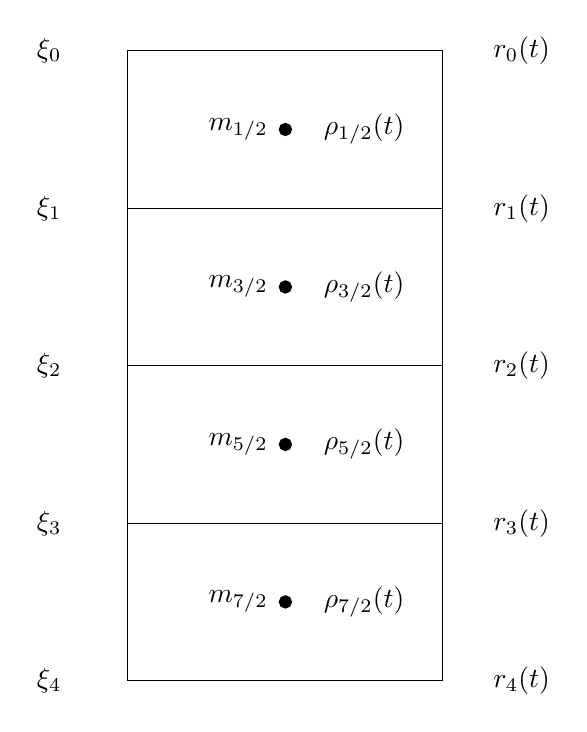
\begin{tikzpicture}[scale=2]
\coordinate (O) at (0,0);
%\draw[semithick](0,0) -- (4,5);
%\draw[semithick](0,0) -- (-4,5);
%\draw[semithick] (4,5) arc (45:135:6.4031242374328485);
\draw (0,0) rectangle (2,1);
\draw (0,1) rectangle (2,2);
\draw (0,2) rectangle (2,3);
\draw (0,3) rectangle (2,4);
%%%
%\draw (-0.5,2.5) -- (-0.5,4.5);
%\draw (6.5,2.5) -- (6.5,4.5);
% xi labels basic nodes
\node at (-0.5,4) {$\xi_0$};
\node at (-0.5,3) {$\xi_1$};
\node at (-0.5,2) {$\xi_2$};
\node at (-0.5,1) {$\xi_3$};
\node at (-0.5,0) {$\xi_4$};
% xi labels staggered nodes
\node at (0.7,3.5) {$m_{1/2}$};
\node at (0.7,2.5) {$m_{3/2}$};
\node at (0.7,1.5) {$m_{5/2}$};
\node at (0.7,0.5) {$m_{7/2}$};
% rho labels staggered nodes
\node at (1.5,3.5) {$\rho_{1/2}(t)$};
\node at (1.5,2.5) {$\rho_{3/2}(t)$};
\node at (1.5,1.5) {$\rho_{5/2}(t)$};
\node at (1.5,0.5) {$\rho_{7/2}(t)$};
% r labels basic nodes
\node at (2.5,4) {$r_0(t)$};
\node at (2.5,3) {$r_1(t)$};
\node at (2.5,2) {$r_2(t)$};
\node at (2.5,1) {$r_3(t)$};
\node at (2.5,0) {$r_4(t)$};
% staggered points
\draw[black,thick,fill=black] (1,3.5) circle [radius=1pt] ;
\draw[black,thick,fill=black] (1,2.5) circle [radius=1pt] ;
\draw[black,thick,fill=black] (1,1.5) circle [radius=1pt] ;
\draw[black,thick,fill=black] (1,0.5) circle [radius=1pt] ;
\end{tikzpicture}